\chapter{Moving least squares level set smoothing}
\section{Introduction}
As were previously concluded blur level set method requires hight effort to configure all available parameters to match required fluid surface reconstruction quality. Another helpful method comes in mind, which can be applied to correct an implicit ISO-surface such, that the explicit reconstructed surface will be smoothed out.\\
Moving Least Squares (MLS) is a method for recovering continuous functions from a set of random point samples by calculating a weighted least squares measure biased toward the area around the point at which the retrieved value is requested. Holding in mind, that scalar distance field is the implicit function of the distance to surface, it can be assumed that in the small local neighborhood the function should fit an elementary surface e.g. sphere.\\
In the work \cite{Apss} new Point Set Surface (PSS) definition based on moving least squares (MLS) fitting of algebraic spheres is presented. The central advantages of APSS approach compared to existing planar MLS include significantly improved stability of the projection under low sampling rates and in the presence of high curvature. \textcolor{red}{TODO: add more descriptions}\\
Another important work was performed in \cite{PssLkr} \textcolor{red}{TODO: add description of the work}.\\
In this thesis MLS was applied directly on the SDF. As a blur level set method the level set mls correction method is also developed to be able to apply it on every reconstruction approach, which in the core uses an implicit SDF ISO-surface.  
\section{Moving least squares}
In this section concept of the Moving Least Squares (MLS) will be described. The MLS approximation was introduced in an early paper by Lancaster and Salkauskas  \cite{MLSSalkauskas} in 1981 with special cases going back to McLain  \cite{MLSMcLain1}, \cite{MLSMcLain2} in 1974 and 1976. Since, in MLS one writes the value of the unknown function in terms of scattered data, it can be used as an approximation to span the trial space in meshless (or meshfree) methods. This approximation has found many applications in curve fitting and numerical solutions of partial differential equations.\\
Most of the theoretical material was taken from \cite{MLSIntro}.
\subsection{Global least squares}
\textbf{Problem domain.} Given a points $X = [x_1, ..., x_n]$. The goal of a is to fit point cloud to some geometric surface e.g. sphere. Suppose, that we are given a values of $u(X) = [u_1, ..., u_n]$ and the values are biased, e.g. $u_i + \varepsilon = u(x_i)$ and the function $u(x)$ is unknown.\\ 
The idea of a Global Least Squares (GLS) technique is to reconstruct $u(x)$ so that for all $|u_i - u(x_i)|$ is minimal, that is:
\begin{equation}
	\sum_i (u_i - u(x_i))^2 -> min
	\label{eq:min_problem}
\end{equation}
\textbf{Description.} For simplicity 1D problem will be reviewed e.g. $x_i \in R$. Function $u(x_i)$ can be described as polynomial $u(x)=\sum_k{c_i \cdot x^k}$, where $c_i$ are unknown coefficients, which are to be found.
As soon as in the problem domain $x_i$ are given values we can substitute a $x^k$ with a coefficient $b_k(x) = x^k$. Returning to the equation \ref{eq:min_problem} no the equation can be expanded the minimization problem:
\begin{equation}
	\sum_i (u_i - \sum_j{c_j \cdot b_j(x_i)})^2 = R^{GLS}
	\label{eq:min_problem_exp}
\end{equation}
where $R^{GLS}$ is a function to be minimized. Finding a minimum first derivative of the equation \ref{eq:min_problem_exp} w.r.t. $c_j$ should be taken, and assigned to 0. An example of one derivative over $c_k$ is in Equation \ref{eq:RGLSderivatieve}
\begin{equation}
	\dfrac{\partial R^{GLS}}{\partial c_k} = 2\cdot \sum_i{b_k(x_i) \cdot (\sum_j{b_j(x_i)\cdot c_j} - u_i)} = 0
	\label{eq:RGLSderivatieve}
\end{equation}
or equation \ref{eq:RGLSderivatieve}  can be rewritten as follows:
\begin{equation}
	\sum_i{b_k(x_i) \cdot (\sum_j{b_j(x_i)\cdot c_j})}  = \sum_i {b_k(x_i) \cdot u_i}
	\label{eq:RGLSderFinal}
\end{equation}
Taking all partial derivatives over $c_j$ the set of equations can be generated $LS = 
\begin{matrix}
	\sum_i{b_1(x_i) \cdot (\sum_j{b_j(x_i)\cdot c_j})}  &= \sum_i {b_1(x_i) \cdot u_i}\\
	\sum_i{b_2(x_i) \cdot (\sum_j{b_j(x_i)\cdot c_j})}  &= \sum_i {b_2(x_i) \cdot u_i}\\
	\sum_i{b_3(x_i) \cdot (\sum_j{b_j(x_i)\cdot c_j})}  &= \sum_i {b_3(x_i) \cdot u_i}\\
	...\\
	\sum_i{b_m(x_i) \cdot (\sum_j{b_j(x_i)\cdot c_j})}  &= \sum_i {b_m(x_i) \cdot u_i}\\
\end{matrix}$\\
This is a linear system with m equations and m unknown $c_j$`s. Thus it can be reformulated into a matrix form
\begin{equation}
 B \cdot B^T \cdot c  = B\cdot u
 \label{eq:matrEquation}
\end{equation}
where $B = 
\begin{pmatrix}
	b_1(x_1) & b_1(x_2) & ... & b_1(x_n)\\
	b_2(x_1) & b_2(x_2) & ... & b_2(x_n)\\
	...\\
	b_m(x_1) & b_m(x_2) & ... & b_m(x_n)\\
\end{pmatrix}$, $u = \
\begin{pmatrix}
	u_1\\
	u_2\\
	...\\
	u_n
\end{pmatrix}$ is a vector of the given scalar function values, and $c = 
\begin{pmatrix}
	c_1\\
	c_2\\
	...\\
	c_m
\end{pmatrix}$ are the unknown coefficients of the searched function. Thus the solution of \textbf{c} can be retrieved by solving a linear system formulated by the matrix equation \ref{eq:matrEquation}.\\
Having obtained the coefficients \textbf{c}, we can then compute the value of the function at any point $x$ in the domain using the equation for $u(x)$ . This analysis is substantially unchanged in higher dimensions. An example of a global least squares fit is shown in Figure \ref{fig:gls_example}.
\begin{figure}[H]
	\begin{center}
		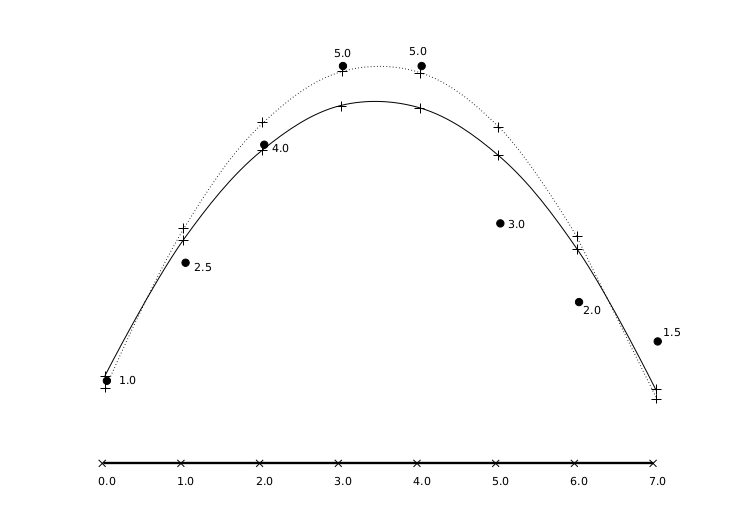
\includegraphics[width=\textwidth]{figures/GLS.png}
	\end{center}
	\caption{Global Least Squares (solid curve) and Weighted Global Least Squares (dashed curve) fit for data represented by the solid circles. The fit is a quadratic fit. The weighting used for the dashed curve is 1.0 every where except at x = 3.0 and x = 4.0 where it is 10.0 (\cite{MLSIntro})}
	\label{fig:gls_example}
\end{figure}
\subsection{Weighted GLS}
\subsection{Weighted Local Least Squares}
\subsection{Moving Least Squares}

\section{Algorithm}
In the Algorithm \ref{alg:mls_alg} general overview of the mls smoothing filter algorithm on MC SDF grid is described. The filter can be applied iteratively, similarly to blur SDF filter. The impact of iterative approach will be described in later section.
\begin{algorithm}[H]
	\scriptsize
	\begin{algorithmic}
		\State generate set of SDF 0-level intersection vertices 
		\State generate neighborClusters form 0-level intersection vertices 
			
		\ForAll{$cluster \in neighborClusters$}
			\State find mls surface approximation for cluster (surfApproximation)
			\ForAll{$vertex \in cluster$}
				\State $newSDF[vertex] \gets newSDF[vertex] + computeUpdatedSDF(vertex, surfApproximation)$
				\State $weights[vertex] \gets weights[vertex] + 1$
			\EndFor
		\EndFor

		\ForAll{$\{vertex, weight\} \in weights$}
			\State $sdfFactor \gets min\left(1, smoothingFactor \cdot \dfrac{fluidParticles[vertex]}{maxFluidParticles}\right)^2$
			\State $newSDF[vertex] \gets sdfFactor \cdot \dfrac{newSDF[vertex]}{weight} + oldSDF[vertex] \cdot (1 - sdfFactor)$
		\EndFor
		\State return levelSet
	\end{algorithmic}
	\caption{mls smoothing filter algorithm}
	\label{alg:mls_alg}
\end{algorithm}
As an input we have an old SDF computed by underlying reconstruction method. From this SDF algorithm detects 0-level intersection vertices (from which final surface vertices will be extracted by linearly interpolating the SDF's between two neighboring vertices with different signs of SDF value). This is required as soon, as the MLS by definition reconstructs surfaces, from SDF that represents a distance to a surface. However, in the used reconstruction methods computed SDF does not represents the distance to a surface along wht whole domain of MC grid. Only the SDF values of 0-level intersection vertices are assumed as a distance to a surface, thus can be used for mls approximation. Intersection cells are shown in the Figure \ref{fig:intersection_vertices}\\
\begin{figure}[H]
	\begin{center}
		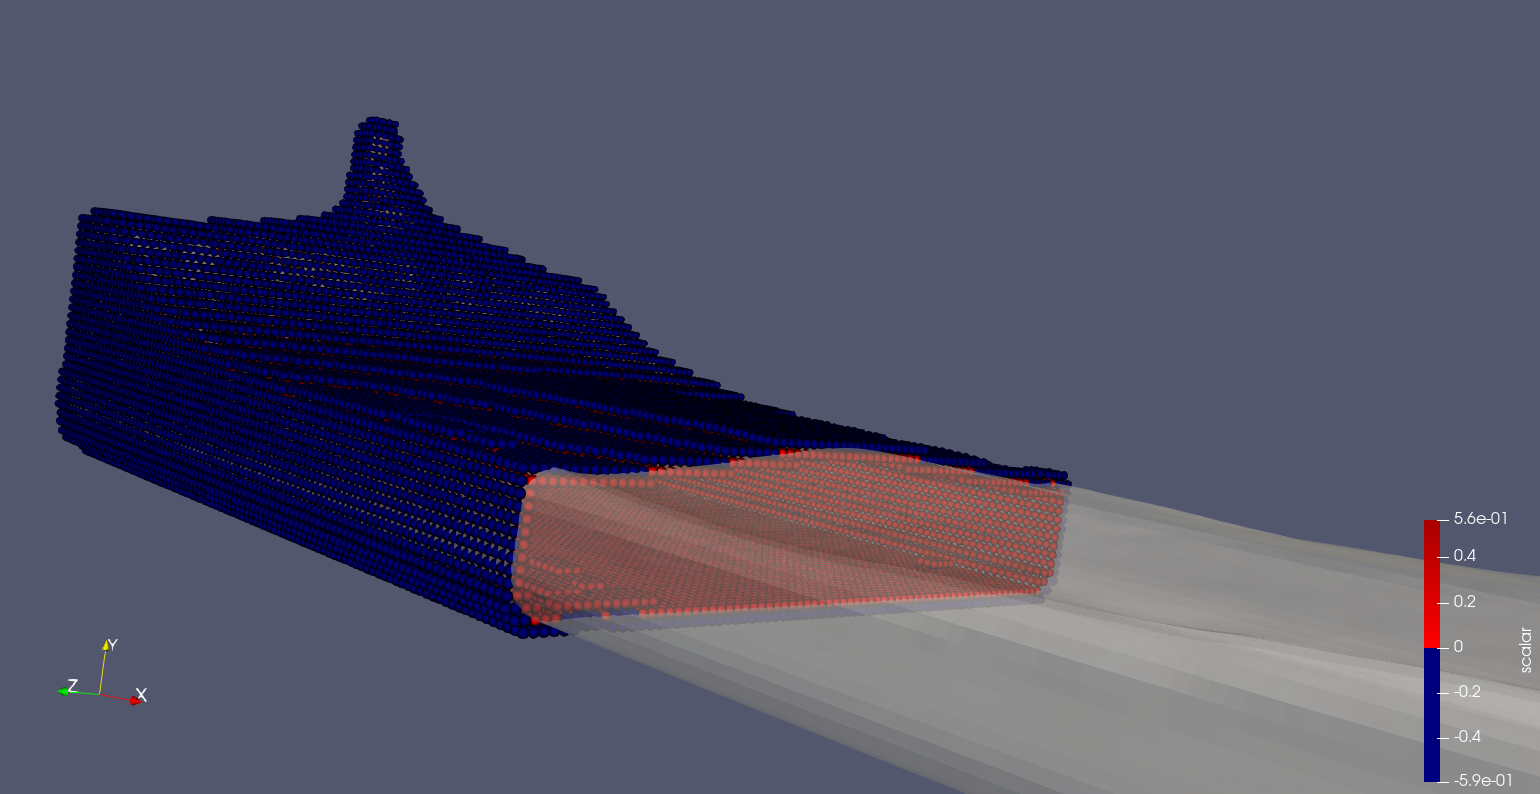
\includegraphics[width=\textwidth]{figures/MlsIntersectionVertexSet.png}
	\end{center}
	\caption{0-level intersection MC grid vertices}
	\label{fig:intersection_vertices}
\end{figure}

Another advantage of using only this set of 0-level intersection vertices is that the algorithm can exactly determine the set of neighbor MC vertices that lie along the reconstructed surface, without approximating the surface normal and taking approximate neighbor set along the tangential direction to the normal. Some computed clusters are represented in the Figure \ref{fig:clusters}\\
\begin{figure}[H]
	\begin{center}
		\begin{subfigure}[b]{0.45\textwidth}
			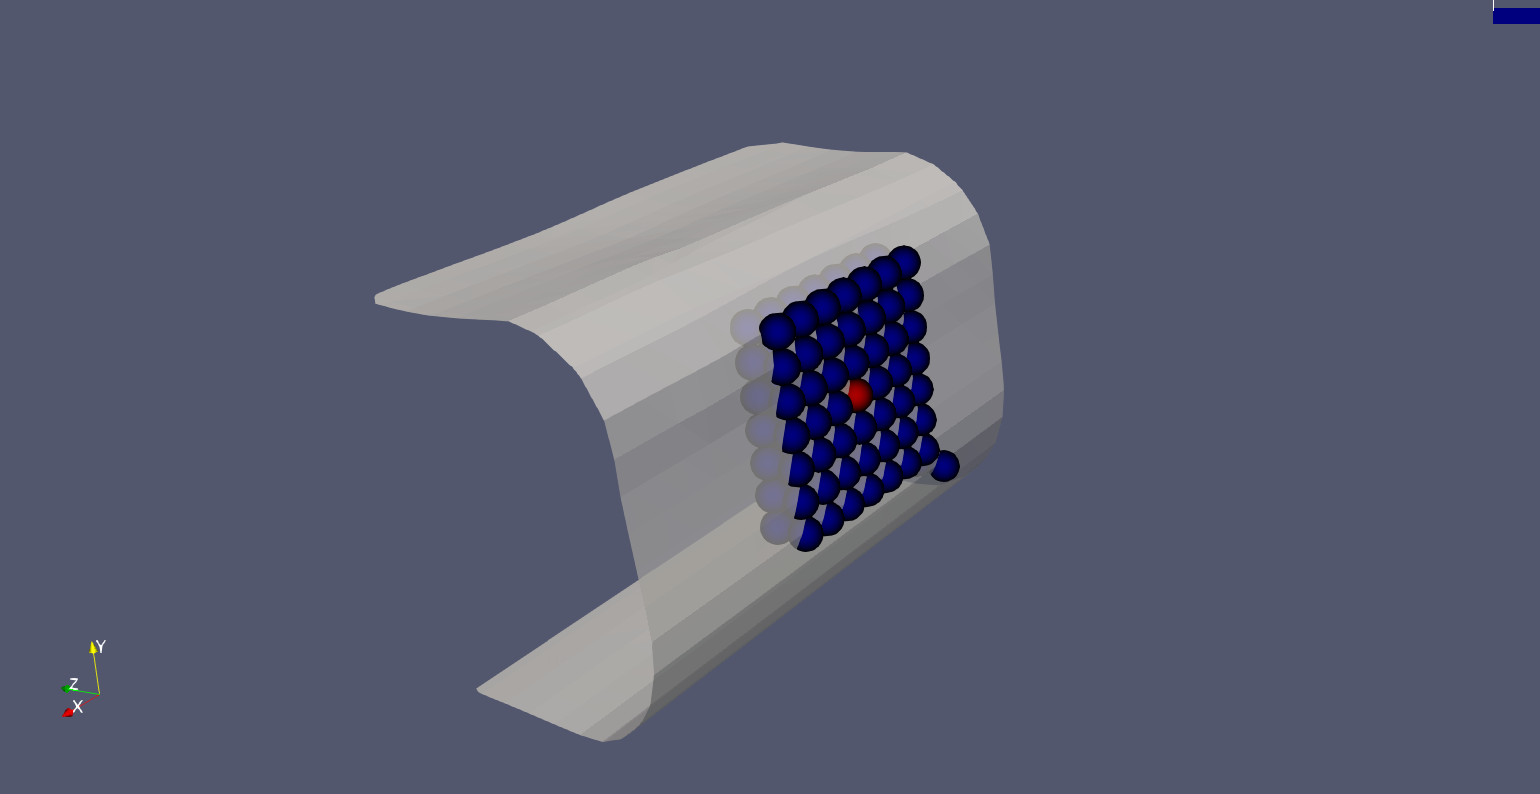
\includegraphics[width=\textwidth]{figures/MlsCluster.png}
		\end{subfigure}
		\begin{subfigure}[b]{0.45\textwidth}
			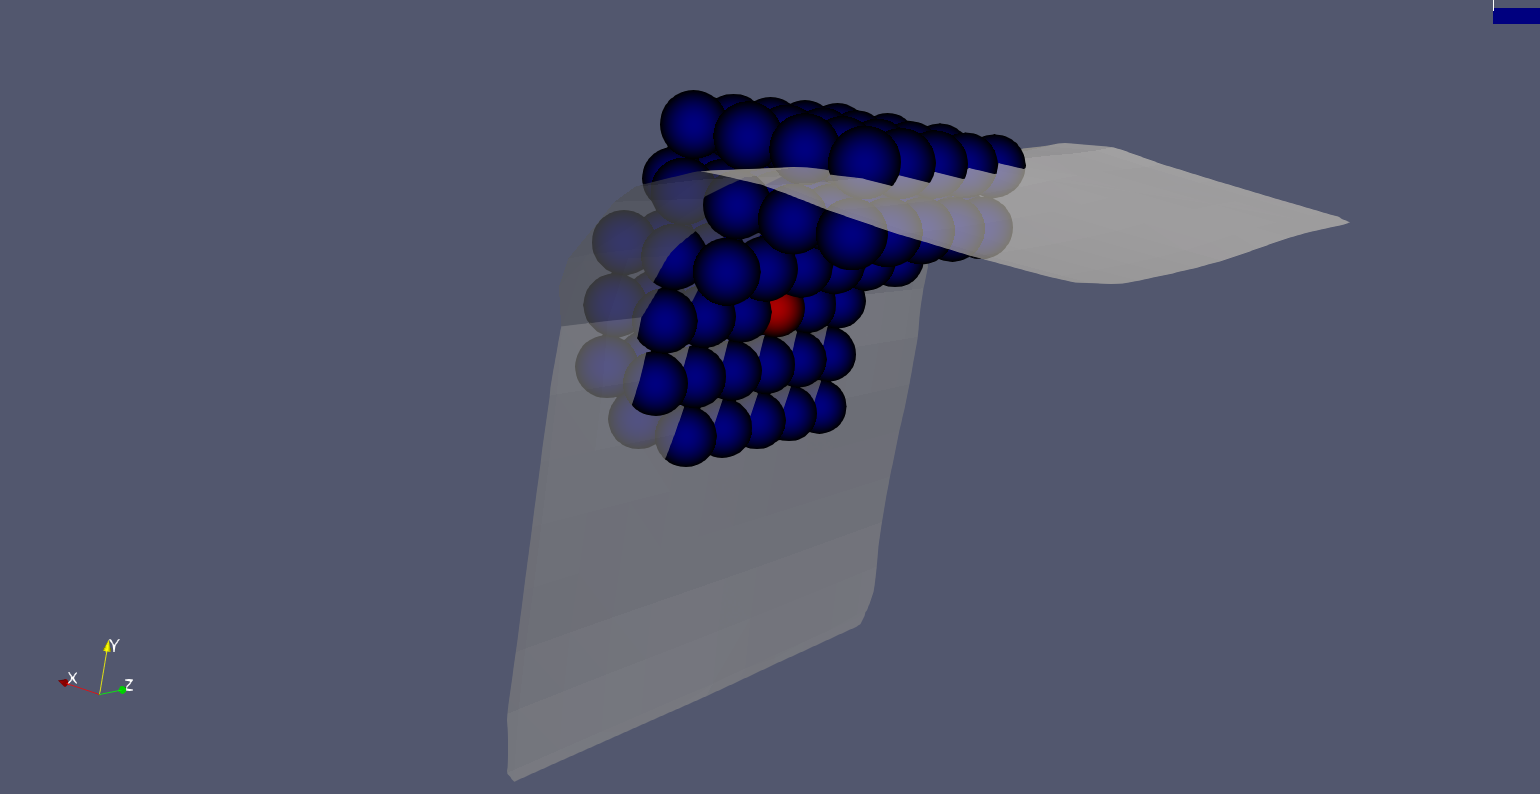
\includegraphics[width=\textwidth]{figures/MlsCluster2.png}
		\end{subfigure}
	\end{center}
	\caption{Examples of computed clusters. Red sphere is a reference vertex, for which cluster is computed.}
	\label{fig:clusters}
\end{figure}

And the last important advantage is a performance influence, as far as there is no need to compute costly mls approximation for MC grid vertices that are not in the SDF 0-level neighborhood.\\

However, there is no guarantee that after the applying approximation the SDF sign of the MC grid vertex will not be switched, e.g. if some MC grid vertex had a positive SDF value before smoothing, after mls approximation it can take a negative value. In this case the set of 0-level intersection vertices set will be changed, and some of the MC grid vertices, that was not mls smoothed will be used during the final surface generation and can bring another noise to the reconstructed surface. This issue can be worked around by applying multiple iteration of mls smoothing trading off final surface smoothness and reconstruction performance.\\

Then clusters are computed, which will be used in the mls approximation. For each cluster coefficients of mls approximated surface is computed, and based on the solution new SDF values are generated for each vertex in the cluster. As soon as vertices can appear in multiple clusters the total values are summed up and then the final value should be divide by a sum of weights. For simplicity and maximization of surface smoothing it was decided to uniformly pick each component of the mls corrected SDF to new corrected SDF from each cluster (all weights of mls corrected sdf values are equal to 1).\\

For thin and small feature areas, where smoothing could bring artifacts, smoothing factor is computed and applied to the final mls value as a weighted sum between the old SDF value and new mls corrected SDF value.\\

\subsection{Clusters computation}
After computing the 0-level intersection vertices of MC grid, clusters are computed. The clusters are a set of neighbor vertices, picked from the 0-level intersection vertices set, which, after all, will be used to compute a mls approximation. The Algorithm \ref{alg:computeClusters} describes the procedure of clusters generation.
\begin{algorithm}[H]
	\scriptsize
	\begin{algorithmic}
			\State $vertices \gets zeroVertexIntersectionCells$
			\While{$vertices$ is not empty}
				\State $vertex \gets vertices.top()$
				\State compute vertex curvature

				\State $maxSamplesFactor \gets \left(\dfrac{min(\dfrac{1}{|curvature|}, fluidParticleDiameter \cdot FluidParticlesCurvatureRadius)}{fluidParticleDiameter \cdot FluidParticlesCurvatureRadius}\right)^2$
				\State $maxSamples \gets MaxSamples \cdot maxSamplesFactor$

				\State $cluster \gets getNeighbourCells(zeroVertexIntersectionCells, vertex, maxSamples)$
				\State $removeParticles \gets max(1, cluster.size() \cdot SampleOverlapFactor)$
				\ForAll{$i \in [0, removeParticles]$}
					\State remove vertex at $cluster[i]$ from $vertices$
				\EndFor
				\State add cluster to clusters
			\EndWhile
			\State return clusters
	\end{algorithmic}
	\caption{mls clusters computation}
	\label{alg:computeClusters}
\end{algorithm}
Here $zeroVertexIntersectionCells$ is a previously computed set of MC grid vertices  that are in the neighborhood of the 0-level SDF,  
$fluidParticleDiameter$ is a diameter of a SPH fluid particles, $FluidParticlesCurvatureRadius$ is a number of particles that can fit in a curvature mean radius (user defined), $MaxSamples$ - user defined maximum number of neighbor vertices, that should be put into a single cluster, $SampleOverlapFactor$ - is a [0, 1] factor measure of how much of a neighbor  vertices within current vertex in the cluster should be removed from the $vertices$ set to avoid re-computation of a cluster for them.\\
Before the algorithm iterates over the vertices in the 0-level intersection vertices set, they are duplicated in separate storage($vertices$). This is required to to be able to remove some of the neighbor vertices from the intersection vertex set to avoid re-computation of the clusters for this vertices, in the mean time to use unchanged set of $zeroVertexIntersectionCells$ in the neighborhood search algorithm. This step adds a trade-off between the reconstruction runtime and surface quality. More explanations will be added in next sections.\\
Next the curvature of the current processed vertex is computed. To save a sharp features of the fluid surface it was decided to decrease the number of neighbors in the cluster, for which mls approximation will be applied. Based on the mean curvature of current 0-level intersection vertex number of samples in the cluster is computed. The curvature is computed using the method described in \cite{CurvatureComputation}. firstly compute the curvature for each surface particle that resides in
this cell with the help of its neighboring particles as:
\begin{equation}
	c_i = \sum_j{(1 - n_i \cdot n_j)\cdot k_c(x_i-x_j, h)}
\end{equation}
where $j$ stands for the neighboring particles, $n_i, n_j$ is the normal of any particle and
$k_c$ is the kernel function described as:
\begin{equation}
	k_c(x_i-x_j, h) = max\left(0, \dfrac{1 - |x_i - x_j|}{h}\right)
\end{equation}
Finally, the curvature of any surface cell is approximated as:
\begin{equation}
	c_{cell} = \dfrac{\sum_i{c_i}}{N}
\end{equation}
where i and N represent the surface particles and the total number of surface
particles inside the cell, respectively.\textcolor{red}{TODO: add picture of the computed maxSamplesFactor}

\subsection{MLS neighborhood search}
Neighbors detection is described in pseudo-code of Algorithm \ref{alg:mls_nbsearch}
\begin{algorithm}[H]
	\scriptsize
	\begin{algorithmic}
		\State push $BaseMcVertex$ to $todoMlsVertices$
		\While{$sizeof(neighborCells) < MlsSamples \land todoMlsVertices \ne \emptyset$}
			\State $currentMcVertex \gets todoMlsVertices[0]$
			\State $todoMlsVertices \gets todoMlsVertices \ todoMlsVertices[0]$
			\If{$indexOf(currentMcVertex) \in SelectedIndices \lor SelectedIndices = \emptyset$}
				\State push currentMcVertex back to neighborCells
			\EndIf
			\ForAll{ $nc \in nearest neighbors of currentMcVertex$}
				\If{$nc \in ZeroLevelIntersectionVertices \land nc \not\in neighborCells \land nc \not\in todoMlsVertices$}
					\State push $nc$ back to todoMlsVertices;
				\EndIf
			\EndFor
		\EndWhile
		return neighborCells;
	\end{algorithmic}
	\caption{mls MC vertex neighbors search}
	\label{alg:mls_nbsearch}
\end{algorithm}
As an input algorithm procedure receives a  $BaseMcVertex$ - a MC vertex for which neighborhood is going to be detected, $ZeroLevelIntersectionVertices$ - 0-level intersection MC vertices which was explained above and $SelectedIndices$ - a set of indeces of neighbors, that should be accepted as a samples (more explanations are in the next section). The procedure returns a set of MC grid vertices, that are in the nearest neighborhood within a requested $BaseMcVertex$, and which are in a set of 0-level intersection MC vertices. The output array has important some properties, that will be exploited further. First of all the all detected neighbors are stored in the array. The further the neighbor is from the base cell the higher index it has inside the array. Figure \ref{fig:mls_neighbor_alignment} shows the example of alignment of detected 0-level intersection neighbors.\\
\textcolor{red}{TODO: add image of neighbors displacement in the array}
\subsubsection{MlsSamples}
The final neighborhood is formed as an area of MC vertices along the 0-level iso surface. The higher value is set int the MlsSamples the larger area of samples within the requested base sample will be configured and the more smoothing will be applied to the SDF, e.g. some examples of computed neighborhood area depending on a number of MlsSamples and respective reconstructed surface are shown in the figure \ref{fig:mls_sample_areas} and figure \ref{fig:mls_samples_example_surfaces}.
\textcolor{red}{TODO: add figures}
Thus modifying number of mls samples influences the final surface quality, in the meantime it increases computation time of the reconstruction.
\subsubsection{SelectedIndices}
To receive a smooth surface it is required to use a large amount of mls samples in the neighborhood as was already shown in previous section. However, it requires much more computation efforts, to compute approximated mls surface and to correct SDF of 0-level vertices. Thus to reduce computation approach it was decided to apply MonteCarlo approach to pick a subset of samples, that was computed by mls neighborhood search, which uniformly represents initially computed set. The hope is that we will be able to correctly detect a our distribution so that the final surface quality will not be degraded too much and the computation time of the reconstruction phase will be reduced.\\
The first idea that comes to mind is just uniformly pick $n$ samples from the computed mls sample buffer. But in this case we need to uniformly pick samples from each distance from the central sample. The probability of picking samples far away from the base sample is larger then the probability of picking the samples near the base cell, e.g. taking for simplicity circle will be used to show  the probability distribution. Thus the density  function of picking arbitrary point, that lies in radius $r$ from the current point is shown in equation \ref{eq:probability_distr}.
\begin{equation}
	p(r) = \dfrac{2 \cdot \pi r}{\pi \cdot R^2} = \dfrac{2 \cdot r}{\cdot R^2}
	\label{eq:probability_distr}
\end{equation}
where $R$ is a radius to the sphere. In another words talking the probability of picking sample on that lies from the central sample in a distance of $r$ is equal to length of the inner circle with radius $r$ divided by the area of the sphere.
Thus to pick samples from the buffer uniformly w.r.t. the distance from the central sample we have to modify the probability distribution of picking a samples from buffer. Next procedure is applied to pick the sample indeces from the buffer:
\begin{algorithm}[H]
	\scriptsize
	\begin{algorithmic}
			\State $acceptedIndices \gets \{0\}$;
			\State $lowerBound \gets 0$
			\State $upperBound \gets (MlsSamples - 1)$
			\For{$i \in [0, MaxSamples]$}
				\State $offset \gets \dfrac{PickRandom(0, MaxSamples - 1)}{MaxSamples}$
				\State $index \gets lowerBound + offset^2 \cdot (upperBound - lowerBound))$
				\State $currentIndex \gets index$
				\While{$index \in acceptedIndices$}
					\If{$index = lowerBound$}
						\State $index = upperBound$
					\Else
						\State $index \gets index - 1$
					\EndIf
				\EndWhile
				\State $acceptedIndices \gets acceptedIndices \cup index$;
				\If{$index = lowerBound$}
					\State $index++;$
					\While{$index \in acceptedIndices$}
						\State $index++$
					\EndWhile
					\State $lowerBound \gets index$
				\Else 
					\If{$index = upperBound$}
						\State $index--;$
						\While{$index \in acceptedIndices$}
							\State $index--$
						\EndWhile
						\State $upperBound \gets currentIndex$
					\EndIf
				\EndIf
			\EndFor
	\end{algorithmic}
	\caption{random sampling of indices's in the mls neighborhood}
	\label{alg:mls_montecarlo_sampling}
\end{algorithm}
The idea of the algorithm is to generate sample from the sample set, and after that shift the index to the beginning. This way the probability distribution of the picking samples in the buffer will compensate the probability distribution of picking samples from specific distance from the central sample.
% \begin{tikzpicture}
% 	\begin{axis}
% 		\addplot[color=red]{exp(x)}
% 	\end{axis} 
% \end{tikzpicture}
Then the calculated $acceptedIndices$ are used to select samples form the buffer.\\
\textcolor{red}{TODO: comparison figure of full neighborhood, uniformly w.r.t. buffer }\\
\textcolor{red}{TODO: comparison of full set of samples and uniformly picked set of neighbors}\\

\subsection{Mls surface computation}
\textcolor{red}{TODO}
\section{Performance analysis}
\section{Results}
\section{Conclusions}